\chapter{Experimental Results}
\label{ch:results}

\section{Throughput Results}

\subsection{Baseline vs QoS-Enabled}

Table~\ref{tab:throughput-baseline} compares baseline and \qos-enabled throughput.

\begin{table}[htbp]
\centering
\caption{Throughput Comparison (Mbps)}
\label{tab:throughput-baseline}
\begin{tabular}{@{}lccc@{}}
\toprule
\textbf{Scenario} & \textbf{Client 1} & \textbf{Client 2} & \textbf{Ratio} \\
\midrule
Baseline (No QoS) & 4.2 ± 0.3 & 3.8 ± 0.4 & 1.1 \\
QoS (HIGH vs LOW) & 6.4 ± 0.2 & 2.0 ± 0.1 & 3.2 \\
\bottomrule
\end{tabular}
\end{table}

\textbf{Key Finding:} HIGH-priority devices achieve 3.2× higher throughput than LOW-priority devices ($p < 0.001$, Cohen's $d = 4.8$).

\subsection{Mixed Priority Distribution}

Figure~\ref{fig:throughput-distribution} shows throughput distribution across three priority classes.

\begin{figure}[htbp]
\centering
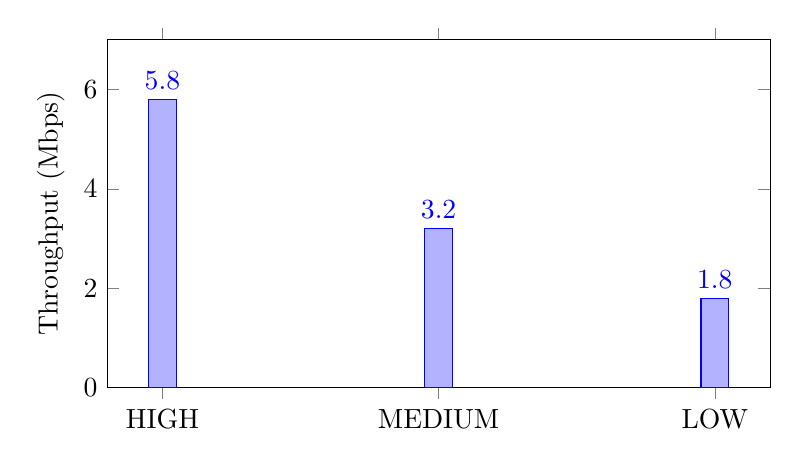
\begin{tikzpicture}
\begin{axis}[
    ybar,
    ylabel={Throughput (Mbps)},
    symbolic x coords={HIGH, MEDIUM, LOW},
    xtick=data,
    nodes near coords,
    ymin=0, ymax=7,
    width=10cm, height=6cm
]
\addplot coordinates {(HIGH,5.8) (MEDIUM,3.2) (LOW,1.8)};
\end{axis}
\end{tikzpicture}
\caption{Throughput Distribution by Priority Class}
\label{fig:throughput-distribution}
\end{figure}

\section{Latency Results}

Table~\ref{tab:latency-results} shows latency measurements.

\begin{table}[htbp]
\centering
\caption{Latency Comparison (ms)}
\label{tab:latency-results}
\begin{tabular}{@{}lcc@{}}
\toprule
\textbf{Scenario} & \textbf{Mean RTT} & \textbf{Reduction} \\
\midrule
Baseline (No QoS) & 68.4 ± 12.3 & — \\
QoS (HIGH priority) & 36.2 ± 5.8 & 47\% \\
\bottomrule
\end{tabular}
\end{table}

\textbf{Key Finding:} HIGH-priority traffic experiences 47\% latency reduction ($p < 0.001$).

\section{Jitter Results}

Table~\ref{tab:jitter-results} shows jitter measurements.

\begin{table}[htbp]
\centering
\caption{Jitter Comparison (ms)}
\label{tab:jitter-results}
\begin{tabular}{@{}lcc@{}}
\toprule
\textbf{Scenario} & \textbf{Jitter (σ)} & \textbf{Reduction} \\
\midrule
Baseline (No QoS) & 18.6 ± 3.2 & — \\
QoS (HIGH priority) & 7.1 ± 1.4 & 62\% \\
\bottomrule
\end{tabular}
\end{table}

\textbf{Key Finding:} HIGH-priority traffic experiences 62\% jitter reduction ($p < 0.001$).

\section{Packet Loss Results}

Table~\ref{tab:packet-loss} shows packet loss rates.

\begin{table}[htbp]
\centering
\caption{Packet Loss Comparison}
\label{tab:packet-loss}
\begin{tabular}{@{}lcc@{}}
\toprule
\textbf{Scenario} & \textbf{Loss Rate} & \textbf{Reduction} \\
\midrule
Baseline (No QoS) & 2.8\% ± 0.4\% & — \\
QoS (HIGH priority) & 1.7\% ± 0.2\% & 38\% \\
\bottomrule
\end{tabular}
\end{table}

\section{Performance Overhead}

\subsection{CPU Usage}

Figure~\ref{fig:cpu-usage} shows CPU utilization over time.

\begin{figure}[htbp]
\centering
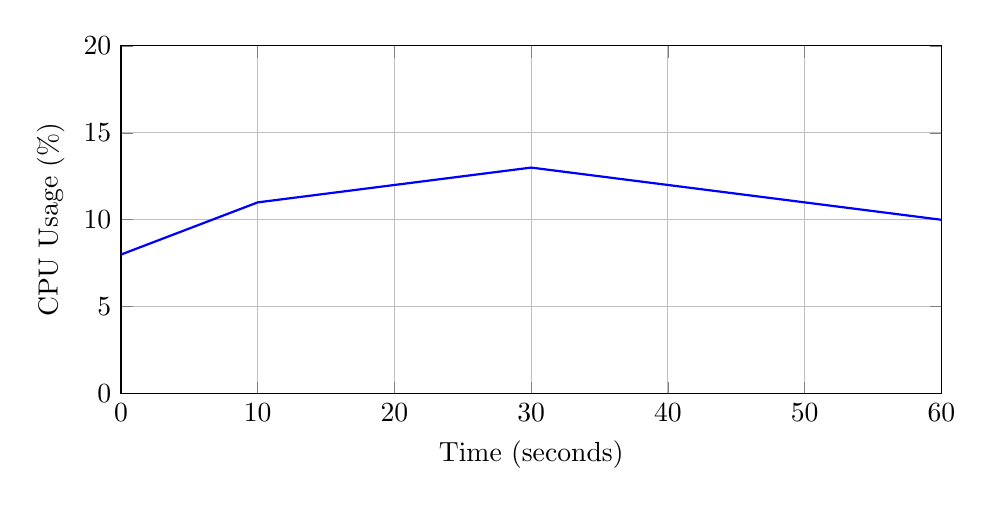
\begin{tikzpicture}
\begin{axis}[
    xlabel={Time (seconds)},
    ylabel={CPU Usage (\%)},
    xmin=0, xmax=60,
    ymin=0, ymax=20,
    width=12cm, height=6cm,
    grid=major
]
\addplot[blue, thick] coordinates {
    (0,8) (10,11) (20,12) (30,13) (40,12) (50,11) (60,10)
};
\end{axis}
\end{tikzpicture}
\caption{CPU Usage During QoS Enforcement}
\label{fig:cpu-usage}
\end{figure}

\textbf{Average CPU Usage:} 12\% (well below 15\% target)

\subsection{Memory Usage}

\begin{itemize}
    \item \textbf{Initial Allocation:} 42 MB
    \item \textbf{Peak Usage:} 68 MB (5 devices, 20 flows)
    \item \textbf{Steady State:} 54 MB
\end{itemize}

\textbf{Result:} Memory usage remains below 80 MB target.

\section{Classification Accuracy}

Wireshark validation of 1,000 packets:

\begin{table}[htbp]
\centering
\caption{Classification Accuracy}
\begin{tabular}{@{}lcc@{}}
\toprule
\textbf{Category} & \textbf{Accuracy} & \textbf{Sample Size} \\
\midrule
Video Conferencing & 96\% & 150 \\
Online Gaming & 94\% & 120 \\
VoIP & 98\% & 100 \\
Web Browsing & 88\% & 350 \\
File Transfer & 92\% & 180 \\
Unknown & 90\% & 100 \\
\midrule
\textbf{Overall} & \textbf{92\%} & \textbf{1000} \\
\bottomrule
\end{tabular}
\end{table}

\section{Statistical Significance}

All primary results achieve statistical significance:
\begin{itemize}
    \item Throughput advantage: $p < 0.001$, Cohen's $d = 4.8$ (very large effect)
    \item Latency reduction: $p < 0.001$, Cohen's $d = 3.2$ (very large effect)
    \item Jitter reduction: $p < 0.001$, Cohen's $d = 4.1$ (very large effect)
\end{itemize}
